
\section{Background}
\subsection{GPU Architecture}
Modern GPUs employ a complex execution pipeline and memory hierarchy to support concurrent execution of parallel threads. 
A typical GPU consists of multiple Streaming Multiprocessors (SMs). 
Each SM includes multiple Single-Instruction-Multiple-Thread (SIMT) units, each of which has multiple lanes of execution. 
Threads scheduled in the same SIMT unit are called a warp, which is the smallest scheduling unit in GPU. 
Like a modern CPU, a GPU consists of multiple memory hierarchies. 
The thread-local registers are the fastest memory component, having the lowest access latency (1-2 cycles). 
The SM local L1 caches and shared memory provide a larger storage capacity over the thread-local registers but have modestly higher accessing latency of around 30 cycles \cite{mei2016dissecting,jia2018dissecting}. 
All the SMs share a unified L2 cache that provides an accessing latency of about 200 cycles. 
The off-chip global memory, similar to the RAM in a CPU system, provides the largest memory storage capacity on the GPU but has the longest accessing latency of around 500 cycles. 
Local memory resides in global memory and is used to hold variables with dynamic indexing or too large to fit into registers. 
It has the same access latency as global memory. 
The key to optimizing memory performance is to make use of the fast memory sub-systems (i.e., registers and shared memory) and reduce the number of memory accesses or transactions. 
Our work is designed to provide such capabilities for convolution operations.

\subsection{Convolution Operations}
Our work targets depthwise separable convolution which contains depthwise convolution and pointwise convolution. 
Depthwise convolution takes as input a 2D feature map and a bank of 2D filters. Each filter is convolved with the corresponding input channel to produce one output channel. 
In the pointwise convolution, all filters are used to convolve with the same input feature map to compute one output feature map. It is the same as multi-channel 2D convolution with the difference that all filters are $1 \times 1$.

When applying quantization to convolutions, the inputs and filters are converted from 32bit floating point (FP32) numbers to 8bit integer (INT8) numbers. 
Channels are accumulated to 32bit integers using $\_\_dp4a$ instructions provided by CUDA \cite{cudatoolkit}.
The final results are converted back to FP32 numbers and written into global memory. 
In this work, we focus on post-training quantization \cite{fang2020post,jacob2018quantization}, which converts the filters of a pre-trained CNN model to INT8 integers offline and the inputs to INT8 integers on-the-fly.

\begin{figure}[t!]
\centering
  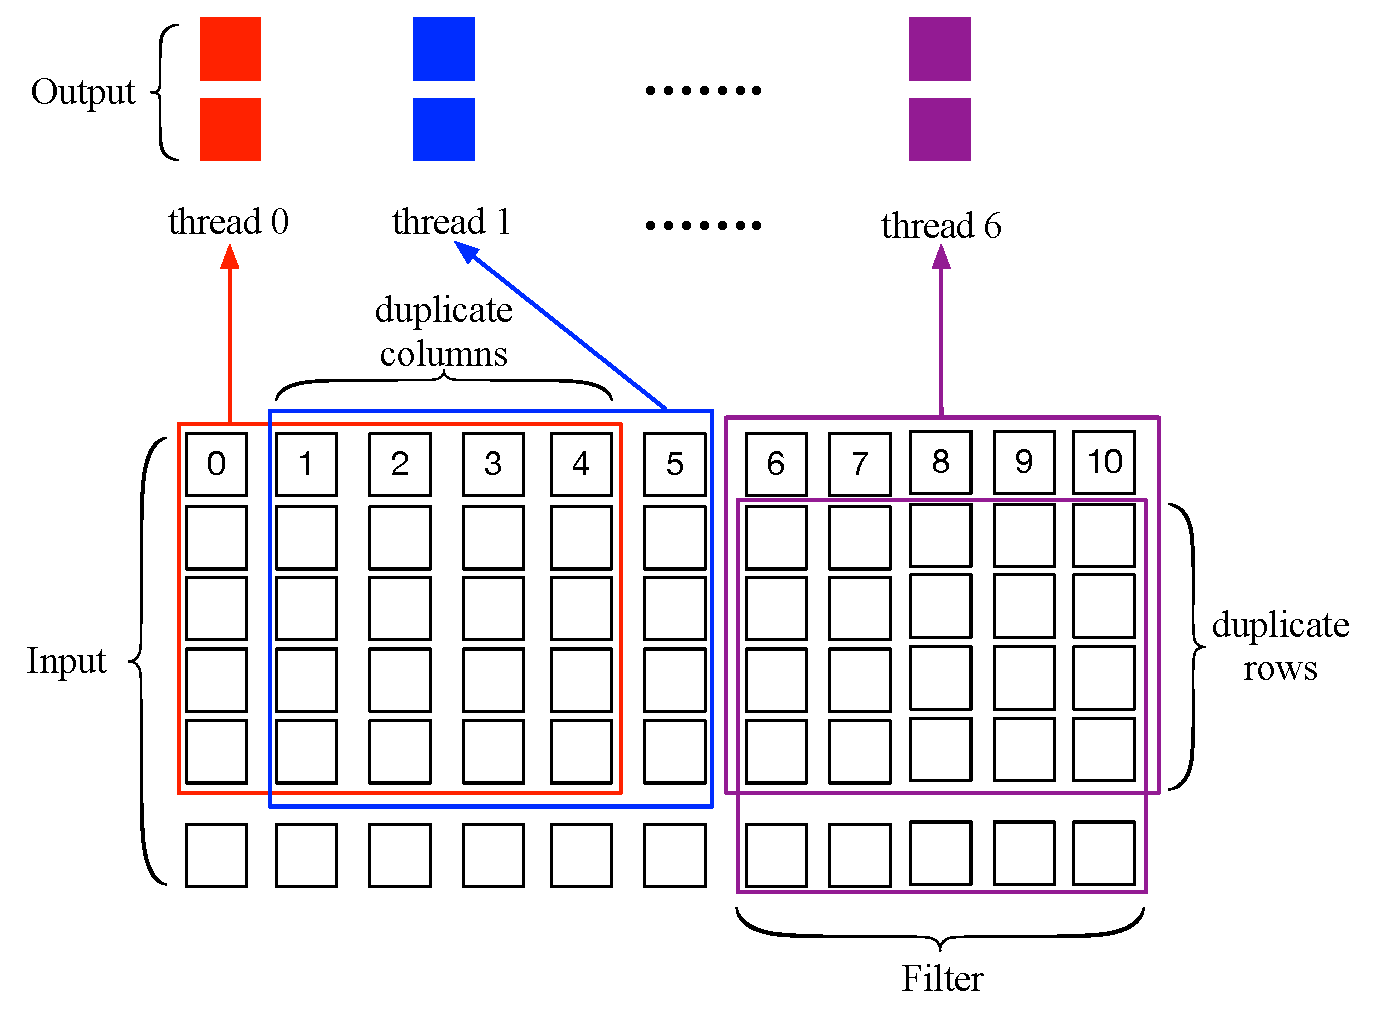
\includegraphics[width=0.9\columnwidth,height=5.5cm]{./figure/twostrategies.eps}
  \caption{Example of performing a single-channel depthwise convolution using a GPU. Here, the filter size is $5 \times 5$, the input image size is $6 \times 11$
  and the output size is $2 \times 7$.}
  \label{fig:twostrategies}
\end{figure}
